\chapter{疾病鉴别诊断的原则和方法}

内科是各临床科室的基础,与各临床科和基础医学有密切的联系。内科诊断技术的发展又能促进其他临床科和基础医学的发展。疾病诊断是否准确和迅速,最能反映内科工作的质量。内科疾病病种繁多、病情复杂、变化多端,同一种疾病可有多种不同的临床病象,某一临床病象又可见于多种不同的疾病。另外,不少其他科的疾病也往往首先就诊于内科,经内科医生鉴定之后才转送各有关临床科处理。因此,一个内科医生就要熟练掌握诊断学的基础理论、基本知识和基本技能,并在临床实践中不断加以充实和提高,才能及时和准确地作出疾病的诊断,提供疾病的治疗和预防的依据,从而使患者能早日恢复健康。

疾病的诊断过程一般有三个环节:①调查研究,收集完整和确实的诊断资料;②综合和分析资料,建立初步诊断;③有需要时做其他有关的检查,动态临床观察,最后验证和修正诊断。疾病诊断须有广博而精深的医学知识,否则对一些疾病必然茫然无知;此外也要不断地积累临床经验,使处理问题时心中有数,但仍须避免对处理问题时有先入之见。疾病诊断过程大致如图\ref{fig1-1}所示。

\begin{figure}[!htbp]
 \centering
 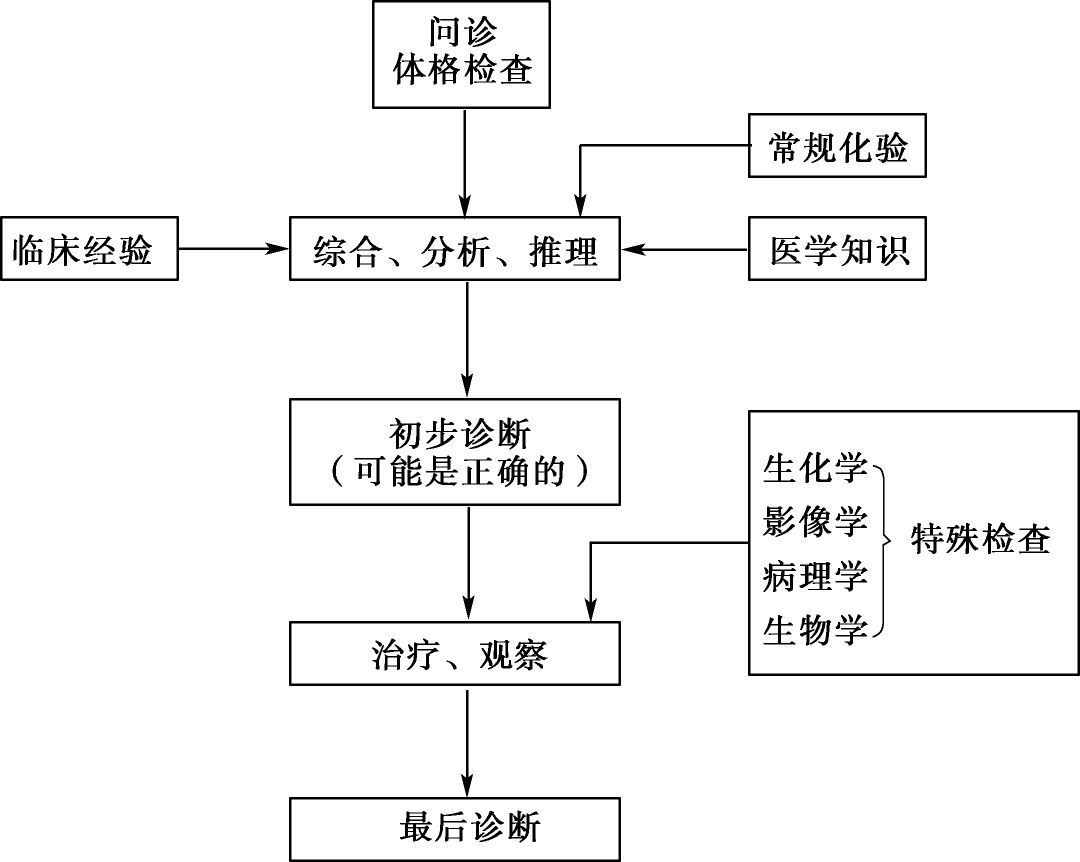
\includegraphics[width=3.80208in,height=2.98958in]{./images/Image00004.jpg}
 \captionsetup{justification=centering}
 \caption{疾病诊断过程图解}
 \label{fig1-1}
  \end{figure} 

\section{一、疾病诊断资料的搜集}

临床医生从检查患者所采得的第一手诊断资料是最宝贵的资料。在对疾病进行调查研究时,掌握的材料必须全面和符合实际,这是取得正确诊断的关键之一。片面的或错误的材料是造成误诊的常见原因。临床材料来自下述三方面:

\subsection{1.完整的病史}

患者叙述的病史可能显得零乱和片段,如果医生采取病史时又带有主观性,则所收集到的病史就难免有片面性和表面性。片面的和不准确的病史会造成诊断上的严重错误,必须注意避免。例如,一个患右下肺大叶性肺炎的患者,以右上腹疼痛、黄疸、发冷、发热为主要症状,但咳嗽轻微,因而就诊时只诉右上腹疼痛、发冷、发热、而未提咳嗽;如果医生思想上主观片面,就可能把注意力错误地放到“急性胆囊炎”上去,而忽视了大叶性肺炎。病史中的一般项目,例如年龄、性别、婚姻、嗜好、月经、职业、发病地区和季节等,与疾病亦可有密切关系,也应重视。例如,一个宫外妊娠破裂的女患者,如果忽视了婚姻史和月经史,医生就容易漏诊。为了采取完整的病史,还要耐心听取患者本人、患者家属、了解病情者和以往经治医生的病情介绍,甚至到患者发病现场调查,全面了解疾病的全过程,才能获得完整的和可靠的病史。

\subsection{2.体格检查}

体格检查必须系统和全面,并取得患者合作,以防止重要的遗漏。例如,一个急性腹痛患者,医生反复在胸部、腹部和腰背部进行检查,均未发现异常,导致得出了一个错误的诊断;以后经过全身细致检查,才发现是腹股沟嵌顿性疝。延误诊断的原因是体检不全面,遗漏了急性腹痛疾病的必要检查所致。由于体检疏忽而误诊,在临床上并非仅仅是个别的例子。

\subsection{3.实验室检查和器械检查}

实验室检查和器械检查要结合临床表现有目的地进行。首先应选用有效而又简便的检查方法。在安排某项检查时,应考虑以下几点:①这项检查的特异性如何?②这项检查的敏感性如何?③检查和标本采集的时机是否合适?能否按规定的要求进行?④标本的输送、检验过程有无误差?⑤患者体质的强弱、病情的起伏、诊疗的处理等对检查结果有无影响?⑥对于可能造成患者负担的检查,例如支气管造影检查和一些负荷试验,还应权衡其利弊并考虑患者能否接受。

实验室检查和器械检查的结果,必须结合临床情况来考虑,才能作出正确的评价。要防止片面依靠实验室检查或器械检查下诊断的错误做法。因而医生就要注意到检查结果有无特异性的问题,以及检查结果的假阳性与假阴性问题。例如,血清甲胎蛋白测定阳性对诊断原发性肝细胞癌有高度的特异性,但仍有少数的原发性肝细胞癌直至临终仍为阴性(假阴性);另一方面,一些非肝癌的疾病却可出现血清甲胎蛋白阳性(假阳性)。实际上,实验室与器械检查的阴性结果,只表明此项检查方法并无阳性发现,而非等同于该被检物的绝对不存在或否定相应疾病的不存在。又因检查时机或技术上的原因,一次、两次实验室或器械检查的阴性结果,往往不足以排除疾病的存在。例如,肾炎的蛋白尿、糖尿病的血糖增高、疟疾的血片中疟原虫等,可以间歇出现;咽拭物白喉杆菌、痰结核杆菌检查的阴性结果,更不容易据以否定有关的疾病。另一方面,粪便培养发现伤寒杆菌或痢疾杆菌,也可见于健康带菌者;肥达试验在一些急性发热性疾病时,其滴度也可以增高。其他如X线检查发现的肺部阴影,超声检查发现的肝区异常波形,均须结合病史、体格检查及其他有关检查才能作出正确的判断。

现代诊断技术有了飞跃的发展,给予临床医生极大的帮助。主要有以下几方面:①内镜的发明与改进;②快速超微量生化学分析技术的应用;③影像学诊断技术的进步;④分子生物学技术的应用;⑤基因诊断赋予遗传病学丰富多彩的内涵。上述各项新型诊断技术的应用,大大地丰富了诊断学的内容,解决了许多临床上的问题。

器械检查可区分为非侵入性(非损伤性)和侵入性(损伤性)两类。原则上应首先采用非侵入性检查。只有当非侵入性检查仍未能明确疾病诊断时,在有明确指征和无禁忌证之下,才选用侵入性检查。

由于尖端诊断技术目前尚未能普及,而大多数的常见病的诊断又不需要复杂的技术进行,因而,临床上我们还须重视诊断疾病时详细询问病史和全面体格检查的基本功,以及结合常规化验和简单的器械检查来进行诊断大多数疾病。

\section{二、建立诊断和验证诊断}

\subsection{(一)整理资料,建立诊断}

\subsubsection{1.努力寻找主要诊断根据}

从调查所得的资料,临床医生须加以筛选、整理、衡量,哪些是主要的,哪些是次要的,并将可疑的材料认真复查、核实,然后将核实的主要材料加以综合分析,弄清它们之间的相互关系,进一步推测病变可能存在的部位(系统或脏器)、性质和病因,为建立正确的诊断打好基础。

有些疾病可出现相当独特的“特殊病征”,如系统性红斑狼疮的蝶形红斑、恙虫病的焦痂、白塞病的口眼外生殖器三联症、麻疹的麻疹黏膜斑、肢端肥大症和库欣综合征的特别面容等。这些“特殊病征”有重要的诊断意义。

又当某些疾病的典型病象已充分显露,出现多个反映该病本质的一组病征时,也有重要诊断价值。如某一患者有阶梯状上升热型、相对性缓脉、蔷薇疹、脾大、血象白细胞减少伴相对性淋巴细胞增多与嗜酸性粒细胞减少或消失,则常可作出伤寒的临床诊断,并进一步作相应的检查加以证实。又如一年轻女性患者,具有不规则发热、多关节痛、肝肾功能损害、血象中等度贫血以及白细胞减少与血小板减少、血沉加快,则可作出系统性红斑狼疮的拟诊,并进一步作狼疮细胞检查及抗核抗体测定以证实之。

疾病的表现各式各样,在不少情况下出现“同病异症”或“异病同症”。例如:急性心肌梗死的患者,多数表现为典型的心前区疼痛,但也可以表现为类似胆石症的上腹部绞痛,甚至可以毫无疼痛,表现为休克或急性充血性心力衰竭,这就是“同病异症”。又如结核病、系统性红斑狼疮、疟疾、钩端螺旋体病、梅毒、白塞病、多发性骨髓瘤、恶性组织细胞病等,可能有多种不同临床表现,类似多种不同的疾病,如不注意可致误诊或漏诊。这些也是“同病异症”的例子。另一方面,如肝大可见于某些寄生虫或细菌、病毒感染的疾病,也可见于肝硬化、肝癌或其他肝病,这就是“异病同症”。例如,阿米巴肝脓肿误诊为肝癌、化脓性心包炎误诊为肝脓肿、轻型地中海贫血误诊为慢性病毒性肝炎,是比较突出的例子。临床上这样的情况有时可遇见,医生要辨别它,就必须进行疾病的鉴别诊断。

在疾病的早期、复杂的或不典型的病例,当找不到可以确定诊断的“特殊病征”时,就要采用下述方法:根据一个主要病征(例如高血压、水肿、血尿等),或先将几个重要的病征组成一个综合征(例如阻塞性黄疸、溶血性贫血等),然后提出一组可能的待鉴别的疾病、进行相互鉴别。在提出一组待鉴别的疾病时,应尽可能将全部有可能性的疾病都考虑在内,以防止严重遗漏而导致诊断错误,这就要求医生要全面考虑问题。但是全面并不等于漫无边际,而是从实际临床材料出发,抓住主要矛盾,提出一组与临床表现相近似的疾病,而且随着分析的深入,相互比较,逐一排除可能性较小的疾病,缩小鉴别诊断的范围,直至留下一个或几个可能性最大的疾病。这就是临床上习称的“排除诊断法”。

对一组疾病进行鉴别诊断时,必然要对组内各个疾病加以肯定或否定。其方法是根据某一疾病本身的特殊点,将其他不相符的近似疾病区别开来,从而达到正确认识疾病。某一疾病的特殊点,我们一般用“诊断根据”的形式加以概括。“诊断根据”一方面包括仅见于该病而不见于其他病的“特殊病征”;另一方面也包括一些并非仅见于该病的病征,但当这些病征与“特殊病征”同时存在时,则能加强“诊断根据”的可靠性。“诊断根据”是从实践中总结得来的,一般来说能够反映疾病的本质,但疾病的表现多种多样,不一定与“诊断根据”完全相符。因此,在运用“诊断根据”时,要紧密联系实际,反对把它作为条条框框,生搬硬套。要将全面的检查材料,参照“诊断根据”,恰当地对病情进行深入的分析,才能得出正确的诊断。例如,胃、十二指肠溃疡合并急性穿孔的“诊断根据”之一是出现膈下游离气影的X线征。但有些胃、十二指肠溃疡穿孔病例,X线检查不一定能查出膈下游离气影。另一方面,在肠气囊肿症时,腹部X线摄片也可见到膈下游离气影,加上此症往往并发于胃十二指肠溃疡,有时可误诊为溃疡病急性穿孔。因此,对急性腹痛患者不能因未发现膈下气影,而认为不完全满足“诊断根据”的要求,便草率排除溃疡病穿孔的可能性,或对胃十二指肠溃疡病患者仅因发现膈下气影,而草率作出溃疡病穿孔的诊断。临床医生应综合全面检查材料加以细致的衡量,有时还需经密切的动态观察才能作出最后的结论。

\subsubsection{2.怎样否定某一疾病}

如拟诊的某一疾病不能解释患者的全部主要临床表现或缺乏预期必定出现的“特殊病征”,则该病可能性很小或可以被否定。前一种情况,例如:两个患者有血尿、膀胱刺激征、尿培养结核菌阳性、静脉肾盂造影显示虫蛀样缺损的X线征,可排除出血性肾盂肾炎,因为用出血性肾盂肾炎不能解释后两种病征,而用肾结核则可全部解释。后一种情况,例如,一个有心前区疼痛的患者,疑有急性心肌梗死,但于三天内反复检查心电图始终正常,血沉加快及谷草转氨酶增高也缺如,则可否定急性心肌梗死的存在。但要注意,有些疾病并无“特殊病征”,或该“特殊病征”只见于疾病的某一阶段,当医生诊治时可能尚未出现或已经消失,后者例如干性心包炎时的心包摩擦音。

\subsubsection{3.怎样肯定某一疾病}

如拟诊的疾病能解释患者的全部主要临床表现,并已找到预期应见于该病的“特殊病征”,例如,拟诊为伤寒的患者血培养发现伤寒杆菌或血清伤寒杆菌凝集试验强阳性,或拟诊为系统性红斑狼疮的患者血中找到狼疮细胞或有高滴度的血清抗核抗体,则可确定各该疾病的诊断。另一方面,当遇到缺乏“特殊病征”的疾病时,一组具有确诊意义的临床综合征也可以起到类似“特殊病征”的作用,但其可靠程度则不及“特殊病征”。例如,根据发热、多关节痛、急性心脏炎、血沉加快和血清抗链球菌溶血素“O”滴度升高等所组成的综合征,大致可诊断为风湿热,但有时仍可与其他结缔组织病相混淆。

在鉴别诊断过程中,经过筛选剩下来几个可能性较大的疾病,要求医生最后肯定一个可能性最大的疾病。这时须注意下述几点:

(1)在几个可能的疾病中进行选择时,一般应先考虑常见病、当地的多发病或当时的流行病。至于罕见病,也应考虑到,但只有用上述疾病不能满意解释患者的临床表现时,才予以考虑。

(2)对患者所患的疾病,在未有充分的诊断根据时不要轻易作出神经症的诊断。

(3)对患者所患的疾病,应先考虑可治之病,其次才考虑不治或难治之病。

(4)当用某种“特殊病征”不能解释某一疾病的全部重要临床现象时,须考虑患者同时存在着两种或多种疾病,或有并发症的存在。

\subsection{(二)临床观察、验证诊断}

疾病是一个或快或慢地运动着的病理过程,在这个过程中,一些临床表现产生了,另一些可能消失了,也可能一个疾病痊愈了,另一个发生了;因此,必须用发展的观点进行分析和诊断。医生每一次的诊查,都只能看到患者疾病全过程中某一阶段的一个横断面,往往要综合多个横断面,才能了解疾病较完整的面貌。这种动态的观察,有助于明确一时未能排除或肯定的疾病的诊断。例如,带状疱疹和麻疹,非候至见疹不易确诊;疑患急性心肌梗死而当时检查心电图未见特异性改变的患者,连续观察几天,并做其他有关的检查,往往即可分晓;热型的动态观察,对于诊断疟疾、回归热等病,有相当大的帮助。

一个正确的认识往往需经反复的实践才能达到。临床医生通过调查研究、收集资料、整理资料、建立诊断之后,工作可告一段落。但工作至此还未结束,更重要的一步是根据诊断进行合理的治疗,治疗效果又反过来验证诊断。如果根据诊断而进行治疗,收到预期的疗效时,那么,一般说来这一诊断工作算是完成了。另一方面,在实践中也不同程度地受着认识水平和技术条件的限制,在这种情况下,部分地或全部的修改原有的诊断是常见的。一些疑难病例往往需要经过深入的动态观察,反复检查,甚至进行诊断性治疗,才能得到正确的诊断。必须强调指出,为了能及时指导防治工作,特别对于急重病例,在临床材料未足以建立确定的诊断之前,也要找出可能性最大的疾病,作为临时诊断,迅速采取治疗措施,同时再进行深入的检查,而不应仅仅纠缠在诊断问题上,以致贻误治疗时机。

\section{三、小 结}

临床医学是一门应用科学,实用为贵。临床医师只有学好和掌握基本功,并在日积月累中进行临床实践和辛勤自学,才能掌握科学、严谨的临床思维方法和诊疗技术,一辈子努力为伤病员服务。

从20世纪末以来,现代化诊断仪器如B超、CT、MRI、电镜等的发明与更新换代,加上分子生物学技术的临床应用,为21世纪的临床医学添加了丰富的内容。可是,必须强调,临床诊断最基本的途径还是全面、细致地应用临床检查方法,包括常规的实验室检查方法,以解决一般的临床问题。一切现代化诊断手段,还须有的放矢地运用,以解决诊断难题,但所得资料仍须和临床资料相结合,才能作出正确的疾病诊断。

一旦实验室检查结果和临床判断不一致,须仔细寻找其原因,直至取得满意的结果。即使结果和临床判断相符,也须在治疗过程中密切动态观察,验证诊断。

再者,由于内科病种繁多,致专业分工越来越细,既有利于提高内科医疗质量,又有利于内科教学和科研的发展,但另一方面又必致形成专科知识强,而大内科知识弱的趋势。因而在疑难病例的处理时,必须加强会诊制度,以期集思广益,交流经验,订好方案,指导临床实践,这才能避免重要疾病的误诊、漏诊和延诊。


\section{参考文献}

1.朱镛连.要注意纠正忽视临床检查倾向.中华内科杂志,1994,33(12):795

2.戴为信.如何选择和分析实验检查结果.中华内科杂志,1998,37(2):134

3.翁心植.大内科面临的挑战.中华内科杂志,1992,31(8):462

4.刘新光.面向新世纪临床医师培养的思考.中华内科杂志,1998,37(1):3


